% \special{dvipdfmx:config z 0} % disable pdf compress to boost compilation time, comment this out for release
\documentclass{article}

\usepackage{amsmath, amsfonts, amsthm, amssymb} 
\usepackage{listings}
\usepackage{graphicx}
\usepackage{float}
\usepackage{subfigure}
\usepackage{geometry}
\usepackage{hyperref}
\usepackage[parfill]{parskip} % no newline indent
\usepackage{enumitem} % enumerate / ordered list
\usepackage{booktabs} % three-line table
\usepackage{array}   % for \newcolumntype macro
\usepackage{listings} % MATLAB code block
\usepackage{pdfpages} % include external pdf pages
\usepackage[bottom]{footmisc} % move footnote to the bottom
\newcolumntype{C}{>{$}c<{$}} % math-mode version of "l" column type

\theoremstyle{definition} % definition
\newtheorem{definition}{Definition}[section]
\newtheorem{theorem}{Theorem}[section]
\newtheorem{remark}{Remark}[section]

\newcommand{\dd}{\mathrm{d}}
\newcommand{\RR}{\mathbb{R}}
\newcommand{\NN}{\mathbb{N}}
\newcommand{\ZZ}{\mathbb{Z}}
\newcommand{\CC}{\mathbb{C}}
\newcommand{\PP}{\mathbb{P}}


\lstset{
  language=Matlab, 
  frame=shadowbox, 
  numbers=left,
  breaklines=true
}

\geometry{
	paper=a4paper, 
	top=2.5cm,
	bottom=2.5cm, 
	left=2.5cm, 
	right=3cm,
	headsep=0.75cm, 
}
\title{ROB 422 HW 4}
\author{Yulun Zhuang \\ \href{mailto:yulunz@umich.edu}{yulunz@umich.edu}}
\date{\today}

\begin{document}

\maketitle

\section*{Questions}
\subsection*{1.}
% TODO Explain why it is more difficult to define a distance metric that leads to good performance for a non-holonomic motion planning problem than a holonomic one. Use a car as an example that illustrates this difficulty and include diagrams.

Defining a distance metric for a non-holonomic system like a car is more complex due to the constraints on its motion. For holonomic system, a widely used distance metric like Euclidean distance assumes that the vehicle can move between arbitrary nearby configurations using a straight line. Since the car cannot move directly to any point between configurations (Figure \ref{fig:nonholonomic}), we need to consider its dynamics and kinematics constraints. Moving between states (with no obstacles) in a non-holonomic system is defined as the two-point Boundary Value Problem (BVP), but this method can only be used locally i.e. small difference between states since it doesn't consider any obstacles and can take a long time to solve for large state difference.


\begin{figure}[H]
    \centering
    \subfigure[Holonomic System]{
        \textsf{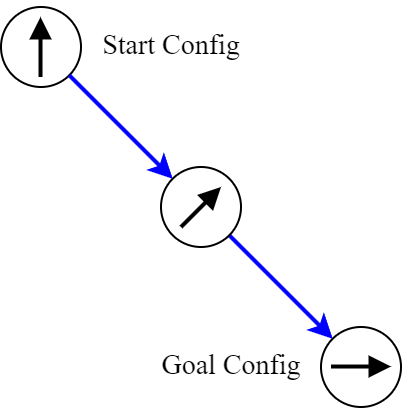
\includegraphics[width=0.3\columnwidth]{holonomic.png}}
    }
    \quad
    \subfigure[Non-holonomic System]{
        \textsf{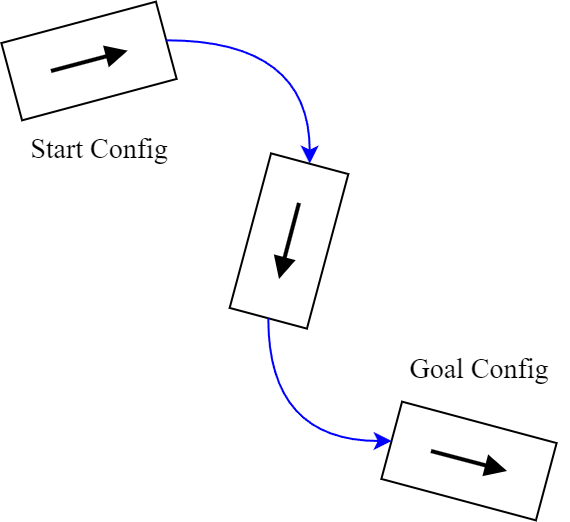
\includegraphics[width=0.3\columnwidth]{nonholonomic.png}}
    }
    \caption{Moving between nearby configurations for Holonomic and Non-holonomic systems}
    \label{fig:nonholonomic}
\end{figure}



\section*{Implementation}

\subsection*{Iterative Inverse Kinematics (IK)}
\subsubsection*{(c)}
\begin{figure}[H]
    \centering
        \textsf{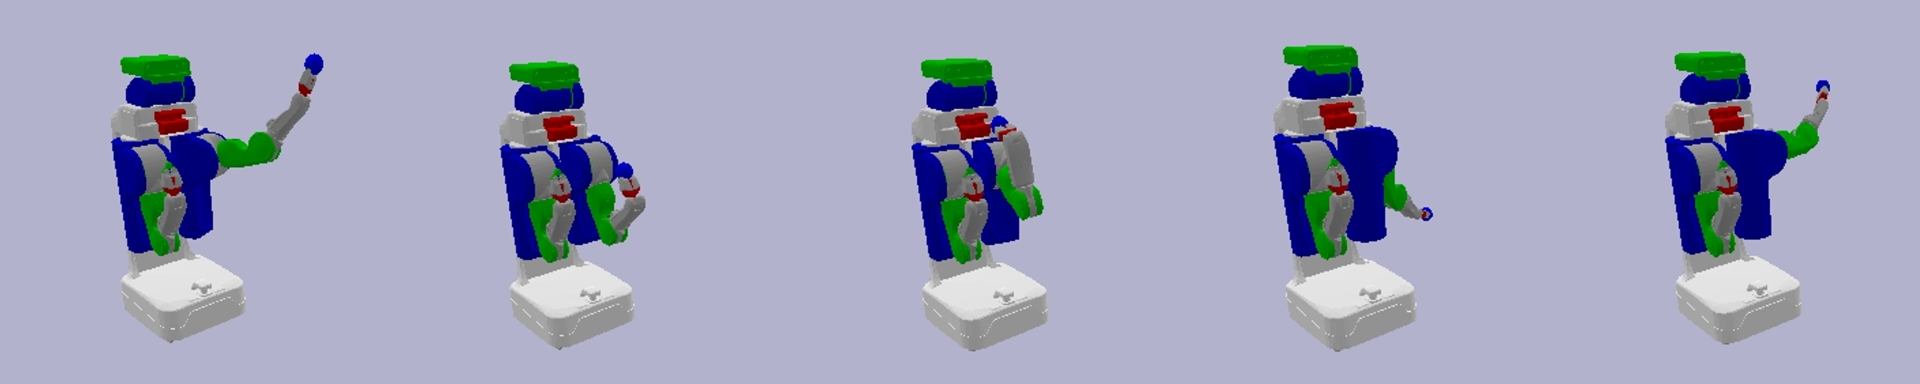
\includegraphics[width=0.9\columnwidth]{ik_target_group.png}}
        \caption{Visualization of the final configurations placed the end-effector at position targets 0 to 4. Configurations solved by iterative IK.}
        \label{fig:ik}
\end{figure}

Configurations that placed the end-effector at target positions
\begin{enumerate}
    \item Reached target 0 in 160 iterations with config:\\
    $[ 0.4392  -0.24767 -0.15007 -0.6481  -0.03273 -0.37433  0.     ]$
    \item Reached target 1 in 253 iterations with config:\\
    $[-0.       1.04887 -0.      -1.82736  0.      -1.33731  0.     ]$
    \item Reached target 2 in 281 iterations with config:\\
    $[-0.22439  0.29065  0.13516 -2.03707  0.05319 -1.15014  0.     ]$
    \item Reached target 3 in 292 iterations with config:\\
    $[ 1.93594  0.96999 -0.      -0.34685 -0.      -0.28347 -0.     ]$
    \item Reached target 4 in 435 iterations with config:\\
    $[ 1.72328 -0.0391  -0.61339 -0.52134 -0.24486 -0.28476  0.     ]$
\end{enumerate}

\subsubsection*{(d)}
\begin{figure}[H]
    \centering
        \textsf{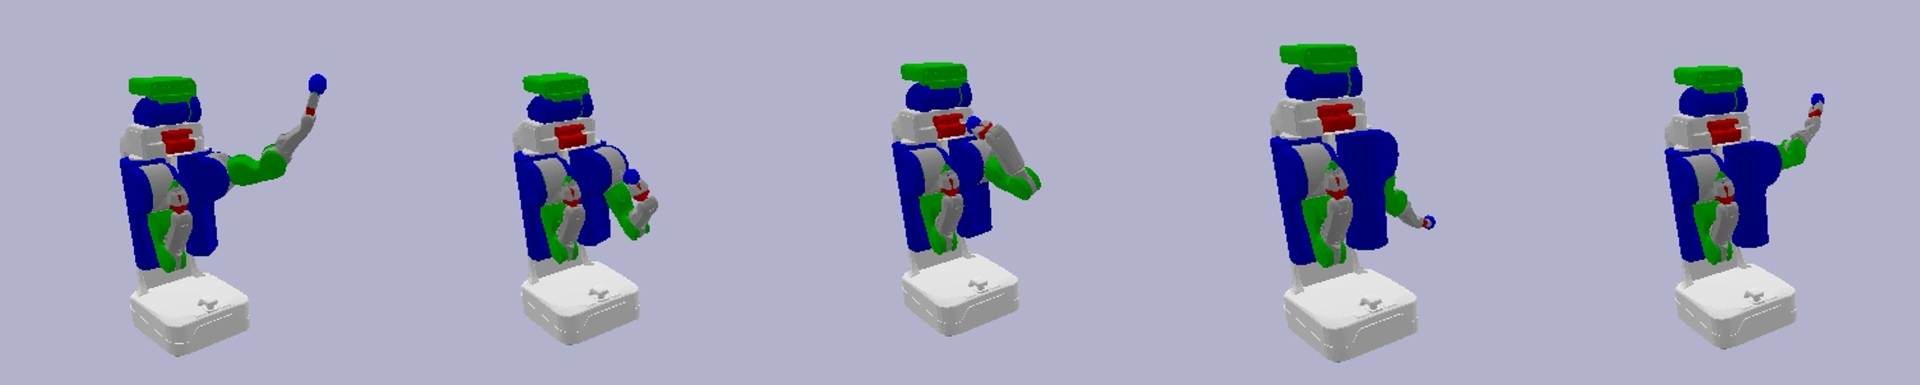
\includegraphics[width=0.9\columnwidth]{ik_null_target_group.png}}
        \caption{Visualization of the final configurations placed the end-effector at position targets 0 to 4 while repelling away from joint limits. Configurations solved by iterative Ik with a secondary task using left null-space projection.}
        \label{fig:ik_null}
\end{figure}

\begin{enumerate}
    \item Reached target 0 in 183 iterations with config:\\
    $[ 0.63309 -0.26777  0.27886 -0.6144  -0.04292 -0.42813  0.     ]$
    \item Reached target 1 in 279 iterations with config:\\
    $[ 0.33772  0.95594  0.48873 -1.78175 -0.00363 -1.38917 -0.     ]$
    \item Reached target 2 in 304 iterations with config:\\
    $[ 0.12212  0.15208  0.48221 -2.00897 -0.02983 -1.15067 -0.     ]$
    \item Reached target 3 in 283 iterations with config:\\
    $[ 1.98607  0.94717  0.22095 -0.28101 -0.07283 -0.3745   0.     ]$
    \item Reached target 4 in 449 iterations with config:\\
    $[ 1.83949  0.02057 -0.20015 -0.49326 -0.24007 -0.3524   0.     ]$
\end{enumerate}


\subsection*{Force Closure Evaluation}
\subsubsection*{(a)}
The volumes for the contact point 1 from Grasp 1 are:
\begin{enumerate}
	\item True volume: 0.1227
	\item 4-vector discretized: 0.0781
	\item 8-vector discretized: 0.1105
\end{enumerate}

The more the number of vectors, the smaller this approximation errors will be, since the approximated shape will get closer to a true friction cone.

\subsubsection*{(b)}
% an explanation of your method for checking force closure and computing the radius of the hypersphere. 

The method for checking force closure:
\begin{itemize}
	\item Input: Contact locations
	\item Output: Is the grasp in force closure? (YES or NO)
\end{itemize}

\begin{enumerate}
	\item Approximate the friction cone at each contact points with a set of wrenches (4-edge or 8-edge polygonal pyramid cone)
	\item Combine wrenches from all cones into a set of	points $S$ in wrench space
	\item Compute the convex hull hull of $S$, and check for each boundary hyperplane, if the plane offset is less than zero i.e. if the origin is inside each half space.
	\item If the origin is inside all half space i.e. the convex hull, return YES. If not, return NO.
	\item If YES, pick the minimum absolute distance from the convex hull to the origin as the maximum hypersphere radius.
\end{enumerate}


% the force closure output for each grasp and the hypersphere radius if the grasp is in force closure. 
The force closure output and hypersphere radius if any:
\begin{enumerate}
	\item Grasp 1: Not in force closure.
	\item Grasp 2: In force closure. Maximum radius: 0.0141 on Mac and Linux; 0.0137 on Windows\footnotemark{}.
\end{enumerate}

\footnotetext{The computation results from Qhull are in little different between Linux and Windows systems, while the same result is achieved on Mac and Linux. Results are tested with the same script but different laptops under the Honor Code.}

% Explain why knowing the hypersphere radius is useful.
Knowing the hypersphere radius is useful because the maximum radius of the hypersphere represents the maximum external disturbance this grasp can resist, i.e. how stable this grasp is.

\subsection*{Principle Component Analysis (PCA)}

\subsubsection*{(a)}
\begin{figure}[H]
    \centering
        \textsf{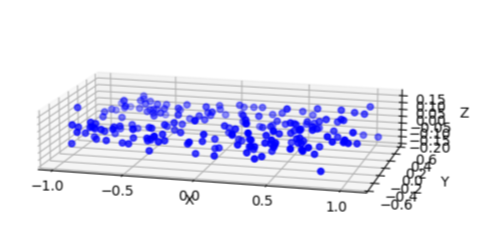
\includegraphics[width=0.5\columnwidth]{pca_rotated.png}}
        \caption{Rotated point cloud that aligns the surface in the point cloud with the XY plane.}
        \label{fig:pca_rotated}
\end{figure}

% V^T:
% [[-0.52935 -0.00254  0.8484 ]
% [-0.05809 -0.99754 -0.03923]
% [ 0.84641 -0.07005  0.5279 ]]
\begin{align*}
	V^T = 
	\begin{bmatrix}
		-0.52935 & -0.00254 & 0.8484\\
		-0.05809 & -0.99754 & -0.03923\\
		0.84641 & -0.07005 & 0.5279
	\end{bmatrix}
\end{align*}

\subsubsection*{(b)}
\begin{figure}[H]
    \centering
        \textsf{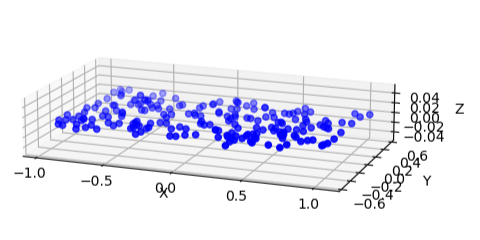
\includegraphics[width=0.5\columnwidth]{pca_projected.png}}
        \caption{Rotated point cloud that aligns the surface in the point cloud with the XY plane while also eliminating the noise in the data (z = 0).}
        \label{fig:pca_projected}
\end{figure}

% Vs^T:
% [[-0.52935 -0.00254  0.8484 ]
%  [-0.05809 -0.99754 -0.03923]]
\begin{align*}
	V_s^T = 
	\begin{bmatrix}
		-0.52935 & -0.00254 & 0.8484\\
		-0.05809 & -0.99754 & -0.03923
	\end{bmatrix}
\end{align*}


\subsubsection*{(c)}
\begin{figure}[H]
    \centering
        \textsf{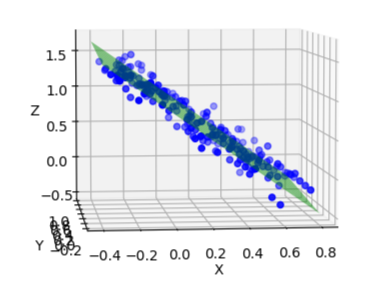
\includegraphics[width=0.6\columnwidth]{pca_plane_fitting.png}}
        \caption{Use PCA to fit a plane (shown in green) to the point cloud.}
        \label{fig:pca_plane}
\end{figure}

The plane normal is $[0.84641,\ -0.07005,\ 0.5279]^T$ with the offset $-0.4549$.


\subsection*{RANdom SAmple Consensus (RANSAC)}

\subsubsection*{(a)}
\begin{figure}[H]
    \centering
        \textsf{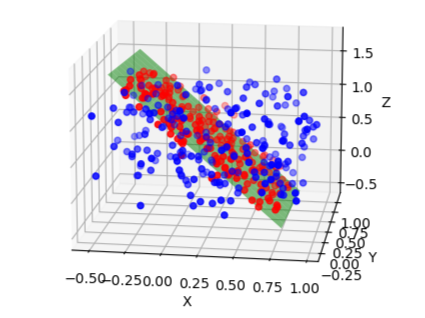
\includegraphics[width=0.6\columnwidth]{ransac_plane_fitting.png}}
        \caption{Use RANSAC to fit a plane (shown in green) to the point cloud. The inliers for the plane are in red, and all other points are in blue.}
        \label{fig:ransac_plane}
\end{figure}

The plane normal is $[0.83917,\ 0.01051,\ 0.54376]^T$ with the offset $-0.54022$.


\subsection*{PCA v.s. RANSAC}

\subsubsection*{(a)}

\begin{figure}[H]
    \centering
    \subfigure[PCA]{
        \textsf{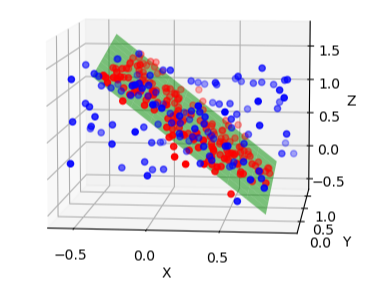
\includegraphics[width=0.46\columnwidth]{semantics_pca.png}}
    }
    \quad
    \subfigure[RANSAC]{
        \textsf{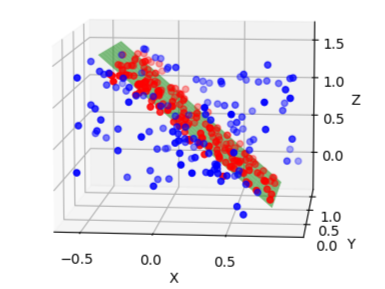
\includegraphics[width=0.46\columnwidth]{semantics_ransac.png}}
    }
    \caption{Comparison of the plane fitting results between PCA and RANSAC. The fitted plane is shown in green, inliers are shown in red and other points are shown in blue.}
    \label{fig:plane_pca_ransac}
\end{figure}


\subsubsection*{(b)}
\begin{figure}[H]
    \centering
        \textsf{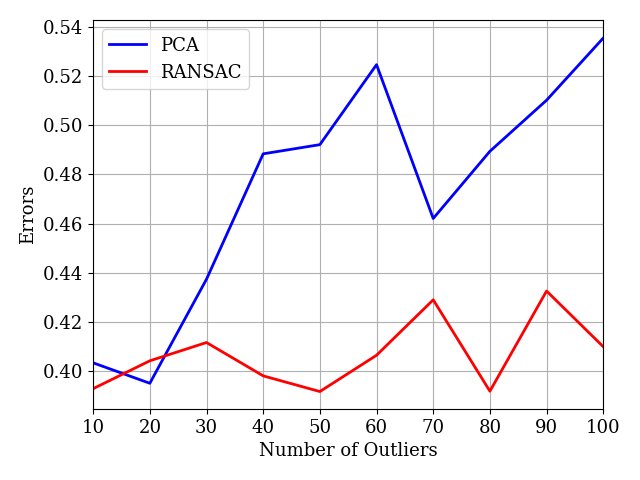
\includegraphics[width=0.6\columnwidth]{pca_vs_ransac.png}}
        \caption{Comparison of inlier fitting errors between PCA and RANSAC as the number of outliers grows.}
        \label{fig:err_pca_ransac}
\end{figure}

The Average computation times of PCA is 0.0017 seconds and that of RANSAC is 0.0686 seconds.

\subsubsection*{(c)}
% Discuss the performance difference between the algorithms. Was there a clear performance difference in terms of computation time and error? If so, which algorithm performed better and why? If not, explain why not.

Overall, RANSAC usually performs better than PCA in terms of fitting errors, while PCA runs much one order of magnitude faster than RANSAC on average. 

RANSAC utilize the random sampling method and use a clear error bound to select inliers and outliers based on sampled model parameters, this technique ensure it to be robust to noise and outliers in the data, but the solution may be sub-optimal and it can run slower due to the number of iterations.

On the other hand, PCA works well when the data has less noise and can run much faster than RANSAC, but as the number of outliers growing, it will perform worse.


\subsection*{Iterative Closest Point (ICP)}


\subsubsection*{(b)}

% Iter: 99 | Errors: 0.01531
\begin{figure}[H]
    \centering
    \subfigure[Registration Result]{
        \textsf{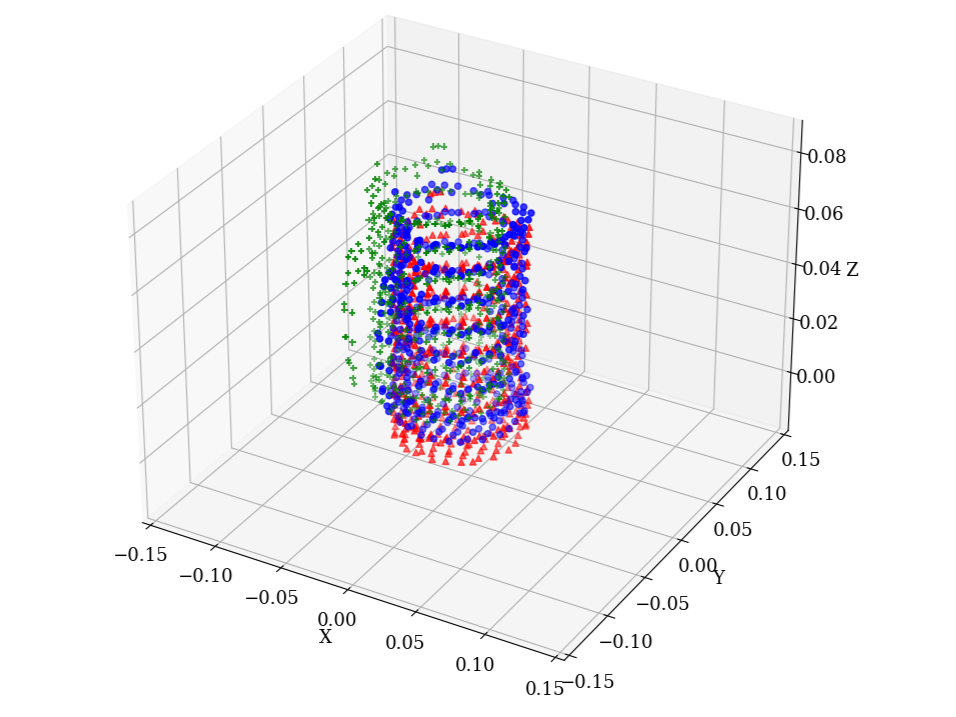
\includegraphics[width=0.46\columnwidth]{icp_align_tgt_0.png}}
    }
    \quad
    \subfigure[Error vs. Iteration]{
        \textsf{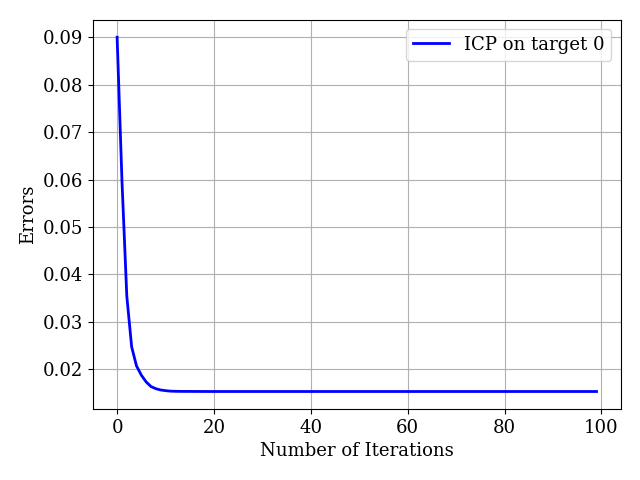
\includegraphics[width=0.46\columnwidth]{icp_err_tgt_0.png}}
    }
    \caption{ICP result for target 0. Source in green, aligned source in blue and target in red.}
    \label{fig:icp_tgt_0}
\end{figure}

% Iter: 31 | Errors: 0.00014
\begin{figure}[H]
    \centering
    \subfigure[Registration Result]{
        \textsf{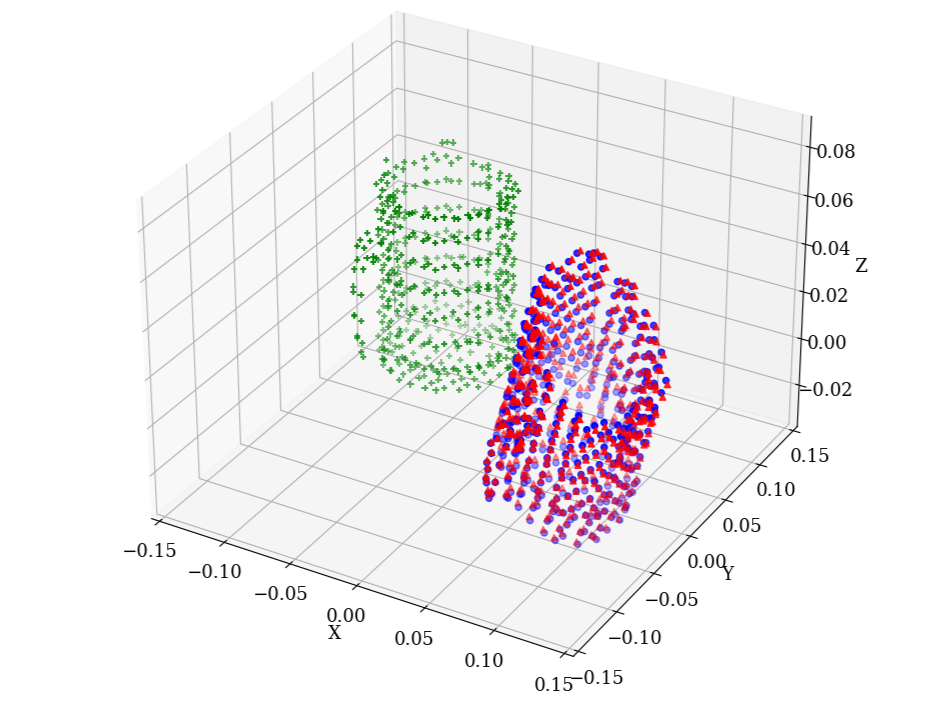
\includegraphics[width=0.46\columnwidth]{icp_align_tgt_1.png}}
    }
    \quad
    \subfigure[Error vs. Iteration]{
        \textsf{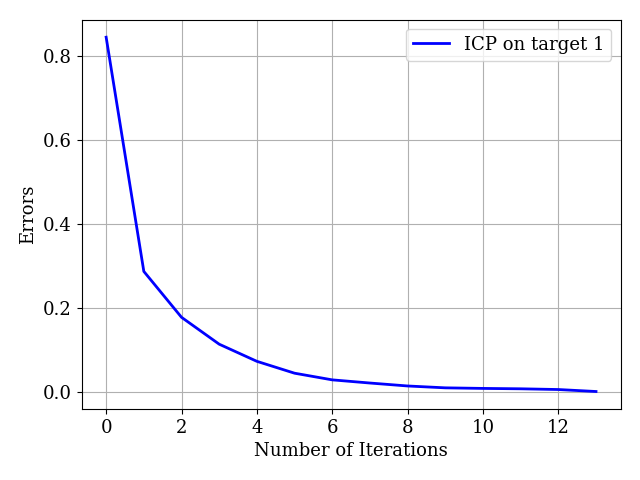
\includegraphics[width=0.46\columnwidth]{icp_err_tgt_1.png}}
    }
    \caption{ICP result for target 1. Source in green, aligned source in blue and target in red.}
    \label{fig:icp_tgt_1}
\end{figure}

% Iter: 99 | Errors: 0.00809
\begin{figure}[H]
    \centering
    \subfigure[Registration Result]{
        \textsf{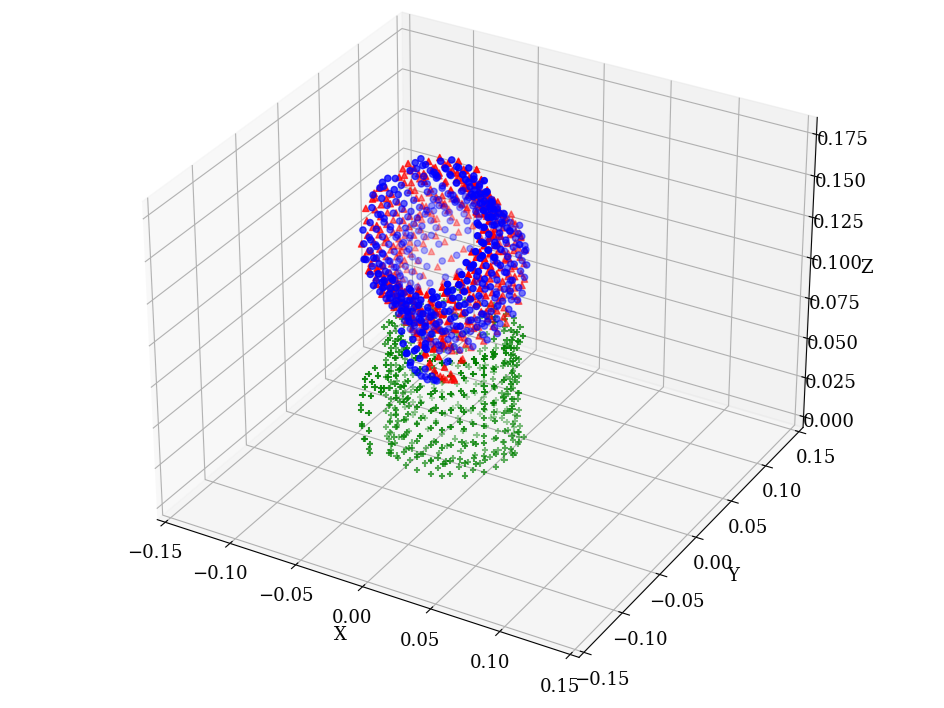
\includegraphics[width=0.46\columnwidth]{icp_align_tgt_2.png}}
    }
    \quad
    \subfigure[Error vs. Iteration]{
        \textsf{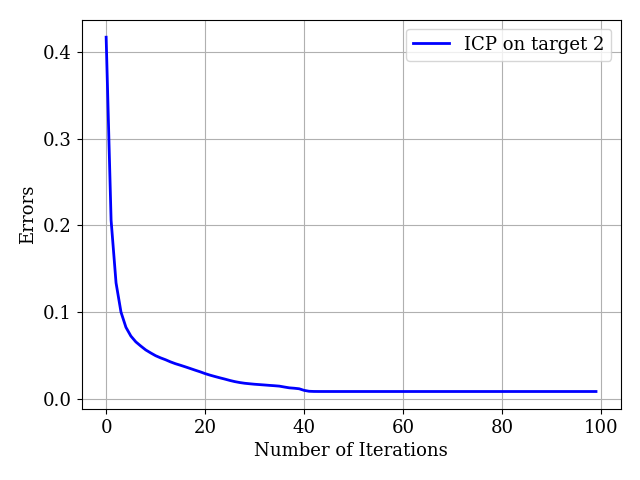
\includegraphics[width=0.46\columnwidth]{icp_err_tgt_2.png}}
    }
    \caption{ICP result for target 2. Source in green, aligned source in blue and target in red.}
    \label{fig:icp_tgt_2}
\end{figure}

% Iter: 99 | Errors: 0.04186
\begin{figure}[H]
    \centering
    \subfigure[Registration Result]{
        \textsf{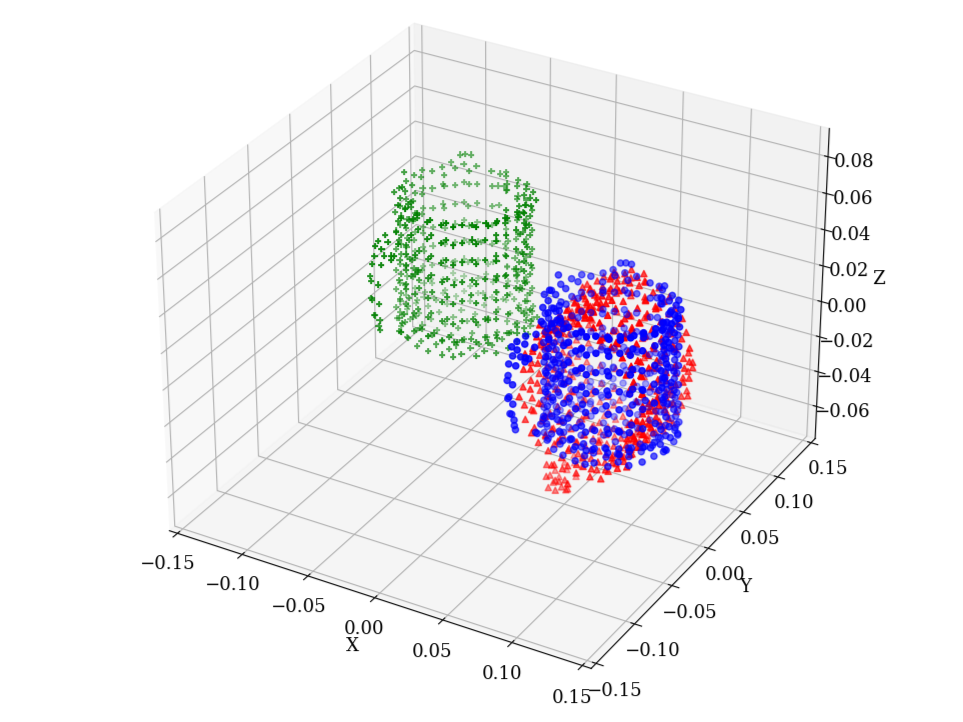
\includegraphics[width=0.46\columnwidth]{icp_align_tgt_3.png}}
    }
    \quad
    \subfigure[Error vs. Iteration]{
        \textsf{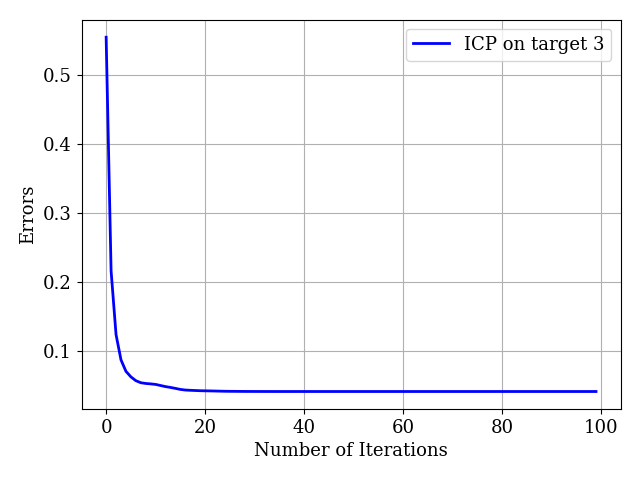
\includegraphics[width=0.46\columnwidth]{icp_err_tgt_3.png}}
    }
    \caption{ICP result for target 3. Source in green, aligned source in blue and target in red.}
    \label{fig:icp_tgt_3}
\end{figure}

\subsubsection*{(c)}
% Discuss the results: which targets were more difficult for ICP and why?
As shown in above figures, target 3 is the most difficult one for ICP. This is because it has a very large orientation difference for the source and target point clouds, and the distance metric we used is just the Euclidean distance. Under this distance metric, it's easy to align the positions of two point clouds, but it's hard to align orientations since it will converge to a sub-optimal closest solution e.g. "embedded" source into target with a totally different orientation (Figure \ref{fig:icp_tgt_3}).


\end{document}